\chapter {Interfacing a Light Dependent Resistor}
\thispagestyle{empty}
\label{ldr}

\newcommand{\LocLDRfig}{\Origin/user-code/ldr/figures}
\newcommand{\LocLDRscicode}{\Origin/user-code/ldr/scilab}
\newcommand{\LocLDRscibrief}[1]{{\tt
    \seqsplit{Origin/user-code/ldr/scilab/#1}},
see \fnrefp{fn:file-loc}}
\newcommand{\LocLDRardcode}{\Origin/user-code/ldr/arduino}
\newcommand{\LocLDRardbrief}[1]{{\tt
    \seqsplit{Origin/user-code/ldr/arduino/#1}},
see \fnrefp{fn:file-loc}}

%%%%%%%%%python
\newcommand{\LocLDRpycode}{\Origin/user-code/ldr/python}
\newcommand{\LocLDRpybrief}[1]{{\tt \seqsplit{%
    Origin/user-code/ldr/python/#1}}, see \fnrefp{fn:file-loc}}
%%%%%%python

%%%%%%%%%julia starts
\newcommand{\LocLDRjuliacode}{\Origin/user-code/ldr/julia}
\newcommand{\LocLDRjuliabrief}[1]{{\tt \seqsplit{%
    Origin/user-code/ldr/julia/#1}}, see \fnrefp{fn:file-loc}}
%%%%%%julia ends

%%%%%%OpenModelica Starts
\newcommand{\LocLDROpenModelicacode}{\Origin/user-code/ldr/OpenModelica}  %added for OpenModelica
\newcommand{\LocLDROpenModelicabrief}[1]{{\tt \seqsplit{%
    Origin/user-code/led/OpenModelica/#1}}, see \fnrefp{fn:file-loc}} % added for OpenModelica

%%%%%OpenModelcia Ends


A Light Dependent Resistor (LDR) or Photoresistor is a light sensitive
semiconductor device whose resistance varies with the variation in the
intensity of light falling on it. As the intensity of the incident
light increases, resistance offered by the LDR decreases. Typically,
in dark, the resistance offered by an LDR is in the range of a few
mega ohms. With the increase in light intensity, the resistance
reduces to as low as a few ohms.   

An LDR is widely used in camera shutter control, light intensity
meters, burglar alarms, street lighting control, automatic emergency
lights, etc. In this chapter we shall interface an LDR with the
\arduino\ board.  

\section{Preliminaries}
A typical LDR and its symbolic representation are shown in
\figref{fig:ldr} and \figref{fig:ldrsym} respectively. The shield
provided with the kit has an LDR mounted on it.  The LDR mounted on
the shield looks exactly like the picture in \figref{fig:ldr},
although, the picture looks a lot larger.  This LDR is connected
to the analog pin 5 of the \arduino\ board. The connections for this
experiment are shown in \figref{fig:ldrconn}. However, the user
doesn't need to connect any wire or component explicitly.

\begin{figure}
\centering
\subfloat[Pictorial representation of an LDR]{
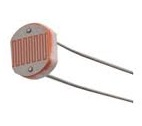
\includegraphics[width=\smfig]{\LocLDRfig/ldr.jpg}
\label{fig:ldr}} \hfill
\subfloat[Symbolic representation of an LDR]{
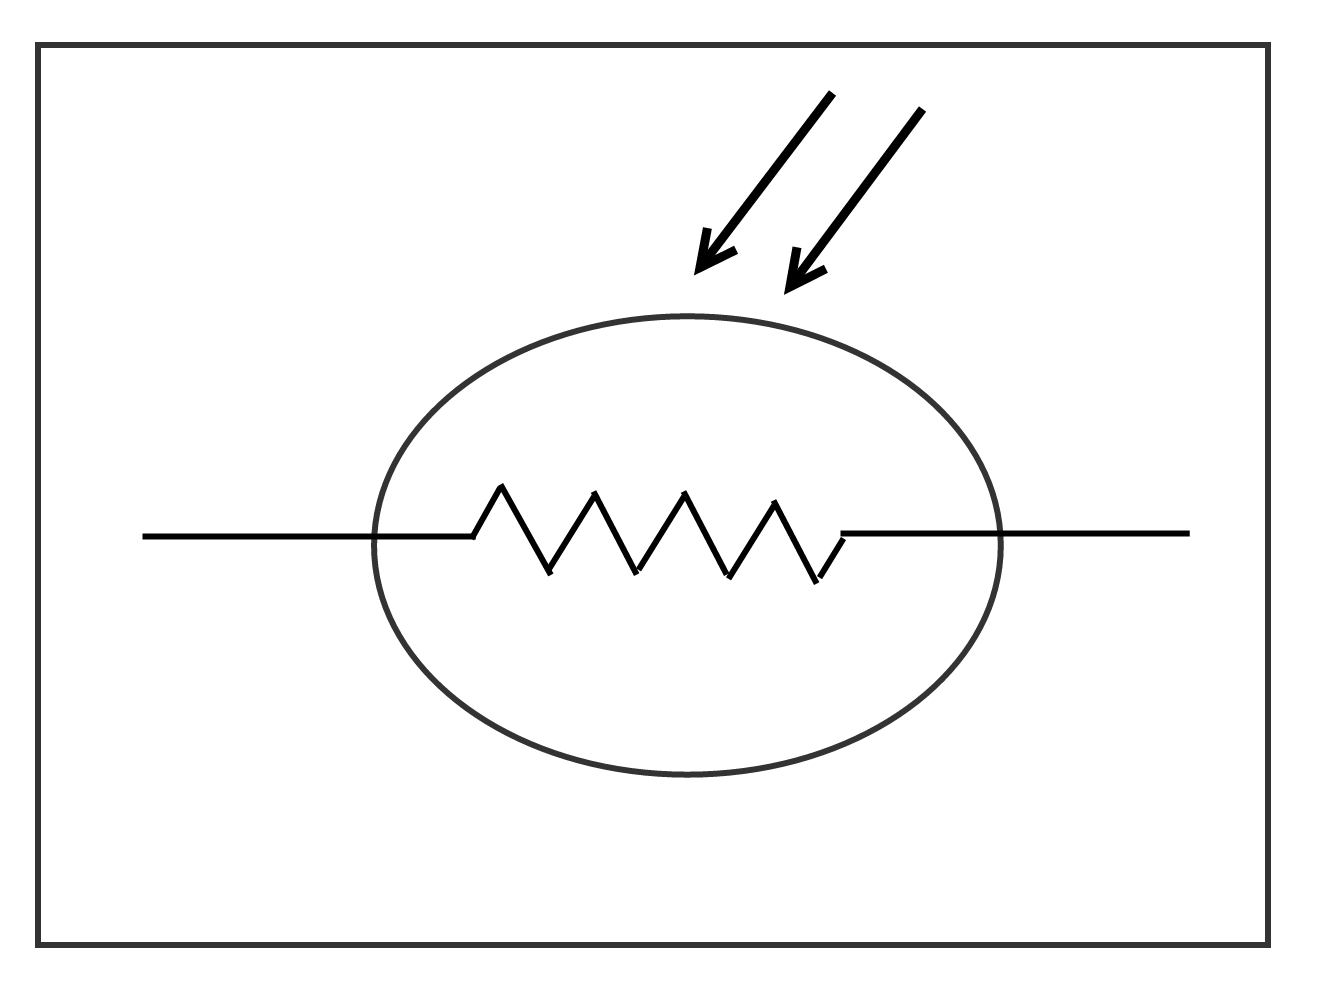
\includegraphics[width=\smfig]{\LocLDRfig/ldr_sym.png}
\label{fig:ldrsym}}
\caption{Light Dependent Resistor}
\end{figure}

\begin{figure}
\centering
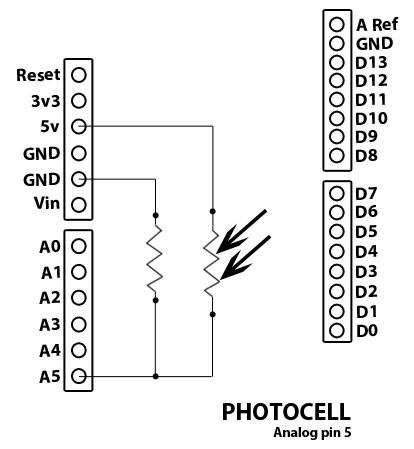
\includegraphics[width=\smfig]{\LocLDRfig/ldr-conn.png}
\caption{Internal connection diagram for the LDR on the shield}
\label{fig:ldrconn}
\end{figure}

The LDR mounted on the shield is an analog sensor. Hence, the analog voltage, corresponding to the changing resistance, across its terminals needs to be digitized before being sent to the computer. This is taken care of by an onboard Analog to Digital Converter (ADC) of ATmega328 microcontroller on the \arduino\
board. ATmega328 has a 6-channel, 0 through 5, 10 bit ADC. Analog pin
5 of the \arduino\ board, to which the LDR is connected, corresponds
to channel 5 of the ADC.  As there are 10 bits, 0-5V readings from LDR
are mapped to the ADC values from 0 to 1023. 

LDR is a commonly available sensor in the market. It costs about
Rs. 100. There are multiple manufacturers which provide commercial
LDRs.  Some examples are VT90N1 and VT935G from EXCELITAS TECH, and
N5AC501A085 and NSL19M51 from ADVANCED PHOTONIX. 

\section{Interfacing the LDR through the Arduino IDE}
\subsection{Interfacing the LDR}
In this section, we shall learn to read the voltage values from an LDR
connected to the analog pin 5 of the \arduino\ board. Later, the read
values will be used to change the state of an LED.   
\begin{enumerate}
\item A simple code to read the LDR values is given in
  \ardref{ard:ldr-read}. As discussed earlier, the 0-5V LDR readings
  are mapped to 0-1023 through an ADC. The 
%\redcolor{Arduino IDE}\ 
  Arduino IDE
  based command for the analog read functionality is given by,
  \lstinputlisting[firstline=6,lastline=6]
  {\LocLDRardcode/ldr-read/ldr-read.ino} where {\tt A5} represents the
  analog pin 5 to be read and the read LDR values are stored in the
  variable {\tt val1}.  The read values are then displayed using,
  \lstinputlisting[firstline=7,lastline=7]
  {\LocLDRardcode/ldr-read/ldr-read.ino} The command, on line 8,
  \lstinputlisting[firstline=8,lastline=8]
  {\LocLDRardcode/ldr-read/ldr-read.ino} is given so that the readings
  do not scroll away very fast.  The entire reading and display
  operation is carried out 20 times.

  To observe the values, one has to open the {\tt Serial Monitor} of
  the Arduino IDE.  The numbers displayed are in the range 0 to 1023
  and depend on the light falling on the LDR.  If one does the
  experiment in a completely dark room, the reading will be 0.  If on
  the other hand, a bright light, say for instance the torch light
  from mobile, is shined, the value displayed is close to 1023.  One
  will get intermediate values by keeping one's finger on the LDR.

\item In this experiment, depending the resistance of the LDR, we will
  turn the red LED on.  The program for this is available at
  \ardref{ard:ldr-led}.  The value of LDR is read and stored in {\tt
    val1}, which is written on to the Serial Monitor.  In case it is
  above some threshold (it is 300 in the code), it puts a high in pin
  number 11.  From \secref{sec:led-pril}, one can see that this pin is
  for the red LED.  If the LDR value is about 300, the red LED will be
  on, else, it will be turned off.  This loop is repeated 2,000 times.
\end{enumerate}

\begin{exercise}
Carry out the following exercise:
\begin{enumerate}
\item Carry out the experiment in a dark room and check what values
  get displayed on the {\tt Serial Monitor}.
\item Carry out the experiment with the torch light from the mobile
  phone shining on the LDR.
\end{enumerate}
\end{exercise}

\subsection{Arduino Code}
\label{sec:ldr-arduino-code}
\addtocontents{ard}{\protect\addvspace{\codclr}}

\begin{ardcode}
\acaption{Read and display the LDR values}
{Read and display the LDR values.  Available at
  \LocLDRardbrief{ldr-read/ldr-read.ino}.}
\label{ard:ldr-read}
\lstinputlisting{\LocLDRardcode/ldr-read/ldr-read.ino}
\end{ardcode}

\begin{ardcode}
\acaption{Turning the blue LED on and off}
{Turning the red LED on and off.  Available at
  \LocLDRardbrief{ldr-led/ldr-led.ino}.}
\label{ard:ldr-led}
\lstinputlisting{\LocLDRardcode/ldr-led/ldr-led.ino}
\end{ardcode}

\section{Interfacing the LDR through Scilab}
\subsection{Interfacing the LDR}
In this section, we will explain a few Scilab experiments to read the
LDR values corresponding to the incident light. The LDR values can be
read using the following function of Scilab Arduino toolbox:
\begin{lstlisting}[style=nonumbers]
  cmd_analog_in(1,port number on Arduino Uno)
\end{lstlisting}
where the input argument 1 is fixed for this kit, and the port number corresponds to the analog pin of \arduino that needs to be read.  We will carry out two experiments using Scilab.

\begin{enumerate}
\item We use \sciref{sci:ldr-read} to read the LDR values.  We find the
  port number from the computer settings and give it as input to the
  {\tt open\_serial} command to start serial port communication. In
  our case, the port number is 2. Next, we shall fetch LDR values
  using the command, {\tt cmd\_analog\_in}, as explained above. This
  is indicated on line 4 of the code. We run this command in a {\tt
    for} loop 20 times. In each iteration of the {\tt for} loop, we
  acquire LDR data fed to analog pin 5, display it in the Scilab
  command window and suspend Scilab operation for 500
  milliseconds. The output of this experiment is displayed on the Scilab command
  window. After reading the values, we close the serial port using the
  command, {\tt close\_serial}, of Scilab-Arduino toolbox.

\item In this experiment, we will observe the saturation point of LDR,
  see \sciref{sci:ldr-led}.  We know that as incident light intensity
  increases, voltage at analog input of the \arduino\ board
  increases. Thus the ADC values being read by the \arduino\ board also
  increase. But after certain high intensity, ADC values reach its
  maximum. For 10 bit ADC in Arduino, this high intensity corresponds
  to 1023.  Beyond this value, the LDR is incapable of sensing the
  change in light intensity and is considered to be saturated. To
  observe this saturation point, we can do a simple task of exposing
  LDR to high intensity. We can put a torch/light source sensor to
  close proximity of LDR.
\end{enumerate}

\begin{exercise}
Carry out the exercise below:
\begin{enumerate}
\item Carry out the exercise in the previous section
\item Calculate the difference in LDR readings in indoor room
  before lighting the lamp and after lighting the lamp. You can also
  record changes in the room lighting at different times of the day.
\end{enumerate}
\end{exercise}

\subsection{Scilab Code}
\label{sec:ldr-scilab-code}
\addtocontents{cod}{\protect\addvspace{\codclr}}

\begin{scicode}
\ccaption{Read and display the LDR values}
{Read and display the LDR values.  Available at
  \LocLDRscibrief{ldr-read.sce}.}
\label{sci:ldr-read}
\lstinputlisting{\LocLDRscicode/ldr-read.sce}
\end{scicode}

\begin{scicode}
\ccaption{Turning the blue LED on and off}
{Turning the blue LED on and off.  Available at
  \LocLDRscibrief{ldr-led.sce}.}
\label{sci:ldr-led}
\lstinputlisting{\LocLDRscicode/ldr-led.sce}
\end{scicode}

\section{Interfacing the LDR through Xcos}
Next, we shall perform the above mentioned experiment, to read LDR
values, through Xcos.  We will carry out the same four experiments as in the previous
sections.  For each, will give the location
of the zcos file and the parameters to set.  The reader should go
through the instructions given in \secref{sec:xcos-start} before
getting started.

\begin{enumerate}
\item The Xcos diagram in \figref{fig:ldr-read} performs data
  acquisition from analog pin 5 and displays the read values on the
  scope.  When the file required for this experiment is invoked, one
  gets the GUI as in \figref{fig:ldr-read}.  In the caption of this
  figure, one can see where to locate the file.

  \begin{figure}
    \centering
    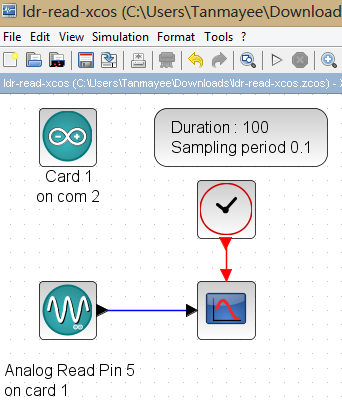
\includegraphics[width=\smfig]{\LocLDRfig/ldr-read-xcos.PNG}
    \caption[Xcos diagram to read LDR values]{Xcos diagram to read LDR
      values.  
      This is what one sees when 
      \LocLDRscibrief{ldr-read.zcos}, is invoked.}
    \label{fig:ldr-read}
  \end{figure}

  We will next explain how to set the parameters for this simulation.
  To set value on any block, one needs to right click and open the
  {\tt Block Parameters} or double click.  The values for each block
  is tabulated in \tabref{tab:ldr-read}.  All other parameters are to
  be left unchanged.
  \begin{table}
    \centering
    \caption{Xcos parameters to read LDR}
    \label{tab:ldr-read}
    \begin{tabular}{llc} \hline
      Name of the block & Parameter name & Value \\ \hline
      ARDUINO\_SETUP & Identifier of Arduino Card & 1 \\
      & Serial com port number & 2\portcmd \\ \hline
      TIME\_SAMPLE & Duration of acquisition(s) & 10 \\
      & Sampling period(s) & 0.1 \\ \hline
      ANALOG\_READ\_SB & Analog Pin & 5 \\
      & Arduino card number & 1 \\ \hline
      CSCOPE & Ymin & 0 \\ 
      & Ymax & 1023 \\
      & Refresh period & 100 \\ \hline
      CLOCK\_c & Period & 0.1 \\
      & Initialisation Time & 0 \\ \hline
    \end{tabular}
  \end{table}

  During this experiment, we vary the light incident on LDR by using
  several light sources and obstacles such as torch light, paper,
  hand, etc. and observe the LDR readings. We observe that with a
  constant light source, the LDR output saturates after some time. 
%The output for this experiment is shown in \figref{fig:ldrsatout}.

%   \begin{figure}
%     \centering
%     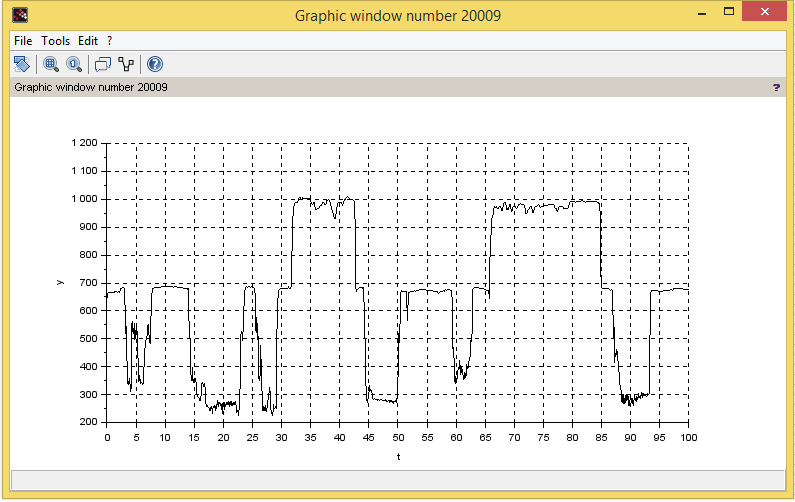
\includegraphics[width=\lgfig]{\LocLDRfig/ldr-sat-out.png}
%     \caption[LDR output for varying intensity of incident light, as
%     seen in Xcos] {LDR output for varying intensity of
%       incident light, as seen in Xcos.  This is what one sees when
%       {\tt \LocLDRscibrief/ldr-read-xcos.zcos} is invoked.}
%     \label{fig:ldrsatout}
%   \end{figure}

\item In the second experiment, we read the value of the LDR and using
  it, turn the red LED on or off.  When the file required for this
  experiment is invoked, one gets the GUI as in \figref{fig:ldr-led}.
  In the caption of this figure, one can see where to locate the file.

  \begin{figure}
    \centering
    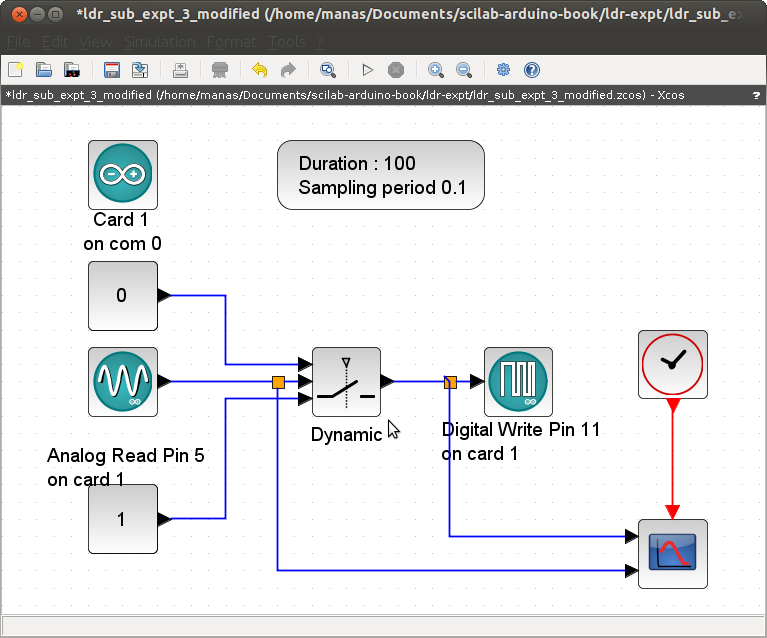
\includegraphics[width=\lgfig]{\LocLDRfig/ldr-led.png}
%    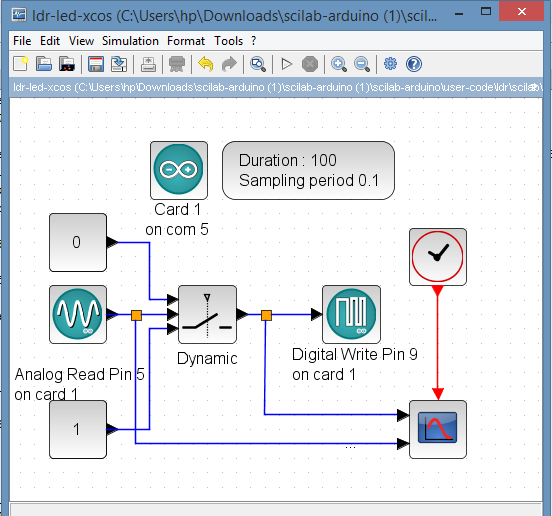
\includegraphics[width=\smfig]{\LocLDRfig/ldr-led-xcos.PNG}
    \caption[Xcos diagram to read the value of the LDR, which is used
    to turn the blue LED on or off] {Xcos diagram to read the value of
      the LDR, which is used to turn the blue LED on or off.  This is
      what one sees when \LocLDRscibrief{ldr-led-xcos.zcos}, is
      invoked.}
    \label{fig:ldr-led}
  \end{figure}

  We will next explain how to set the parameters for this simulation.
  To set value on any block, one needs to right click and open the
  {\tt Block Parameters} or double click.  The values for each block
  is tabulated in \tabref{tab:ldr-led}.  In the CSCOPE\_c block, the
  two values correspond to two graphs, one for digital write and other
  for analog read values.  All other parameters are to be left
  unchanged.
  \begin{table}
    \centering
    \caption{Xcos parameters to read LDR and regulate blue LED}
    \label{tab:ldr-led}
    \begin{tabular}{llc} \hline
      Name of the block & Parameter name & Value \\ \hline
      ARDUINO\_SETUP & Identifier of Arduino Card & 1 \\
      & Serial com port number & 2\portcmd \\ \hline
      TIME\_SAMPLE & Duration of acquisition(s) & 10 \\
      & Sampling period(s) & 0.1 \\ \hline
      ANALOG\_READ\_SB & Analog pin & 5 \\
      & Arduino card number & 1 \\ \hline
      CMSCOPE & Ymin & 0 0 \\ 
      & Ymax & 1 1023 \\
      & Refresh period & 100 100 \\ \hline
      CLOCK\_c & Period & 0.1 \\
      & Initialisation time & 0 \\ \hline
      SWITCH2\_m & Datatype & 1 \\
      & threshold & 300 \\
      & pass first input if field & 0 \\
      & use zero crossing & 1 \\ \hline
      DIGITAL\_WRITE\_SB & Digital pin & 9 \\
      & Arduino card number & 1 \\ \hline
    \end{tabular}
  \end{table}
\end{enumerate}

\section{Interfacing the LDR through Python}
\subsection{Interfacing the LDR}
In this section, we will explain a few Python experiments to read the
LDR values corresponding to the incident light. The LDR values can be
read using the following function of Python Arduino toolbox:
\begin{lstlisting}[style=nonumbers]
  cmd_analog_in(1,port number on Arduino Uno)
\end{lstlisting}
where the input argument 1 is fixed for this kit, and the port number corresponds to the analog pin of \arduino that needs to be read.  We will carry out two experiments using Python.

\begin{enumerate}
\item We use \pyref{py:ldr-read} to read the LDR values.  We find the
  port number from the computer settings and give it as input to the
  {\tt open\_serial} command to start serial port communication. In
  our case, the port number is 2. Next, we shall fetch LDR values
  using the command, {\tt cmd\_analog\_in}, as explained above. This
  is indicated on line 4 of the code. We run this command in a {\tt
    for} loop 20 times. In each iteration of the {\tt for} loop, we
  acquire LDR data fed to analog pin 5, display it in the Python
  command window and suspend Python operation for 500
  milliseconds. The output of this experiment is displayed on the Python command
  window. After reading the values, we close the serial port using the
  command, {\tt close\_serial}, of Python-Arduino toolbox.

\item In this experiment, we will observe the saturation point of LDR,
  see \pyref{py:ldr-led}.  We know that as incident light intensity
  increases, voltage at analog input of the \arduino\ board
  increases. Thus the ADC values being read by the \arduino\ board also
  increase. But after certain high intensity, ADC values reach its
  maximum. For 10 bit ADC in Arduino, this high intensity corresponds
  to 1023.  Beyond this value, the LDR is incapable of sensing the
  change in light intensity and is considered to be saturated. To
  observe this saturation point, we can do a simple task of exposing
  LDR to high intensity. We can put a torch/light source sensor to
  close proximity of LDR.
\end{enumerate}

\begin{exercise}
Carry out the exercise below:
\begin{enumerate}
\item Carry out the exercise in the previous section
\item Calculate the difference in LDR readings in indoor room
  before lighting the lamp and after lighting the lamp. You can also
  record changes in the room lighting at different times of the day.
\end{enumerate}
\end{exercise}

\subsection{Python Code}
\label{sec:ldr-python-code}
\addtocontents{pyd}{\protect\addvspace{\codclr}}

\begin{pycode}
\pcaption{Read and display the LDR values}
{Read and display the LDR values.  Available at
  \LocLDRpybrief{ldr-read.py}.}
\label{py:ldr-read}
\lstinputlisting{\LocLDRpycode/ldr-read.py}
\end{pycode}

\begin{pycode}
\pcaption{Turning the blue LED on and off}
{Turning the blue LED on and off.  Available at
  \LocLDRpybrief{ldr-led.py}.}
\label{py:ldr-led}
\lstinputlisting{\LocLDRpycode/ldr-led.py}
\end{pycode}

\section{Interfacing the LDR through Julia}
\subsection{Interfacing the LDR}
In this section, we will explain a few Julia experiments to read the
LDR values corresponding to the incident light. The LDR values can be
read using the following function of Julia Arduino toolbox:
\begin{lstlisting}[style=nonumbers]
  analogRead(ser,port number on Arduino Uno)
\end{lstlisting}
where the input argument ser give the serial por no. and the 2nd argument gives the Arduino pin to which 
LDR is connected.

\begin{enumerate}
\item We use \juliaref{julia:ldr-read} to read the LDR values. In
  our case, the port number is 2. Next, we shall fetch LDR values
  using the command, {\tt analogRead}. This is indicated in 
  \lstinputlisting[firstline=8,lastline=12]
  {\LocPushjuliacode/led-push-button.jl}. We run this command in a {\tt
    for} loop 20 times. In each iteration of the {\tt for} loop, we
  acquire LDR data fed to analog pin 5, display it in the console. 
  After reading the values, we close the serial port using the
  command, {\tt close}, of Julia-Arduino toolbox.

\item In this experiment, we will observe the saturation point of LDR,
  see \juliaref{julia:ldr-led}.The experiment and its explanation is same 
  as python \& scilab experiment.
\end{enumerate}

\begin{exercise}
Carry out the exercise below:
\begin{enumerate}
\item Carry out the exercise in the previous section
\item Calculate the difference in LDR readings in indoor room
  before lighting the lamp and after lighting the lamp. You can also
  record changes in the room lighting at different times of the day.
\end{enumerate}
\end{exercise}

\subsection{Julia Code}
\label{sec:ldr-julia-code}
\addtocontents{juliad}{\protect\addvspace{\codclr}}

\begin{juliacode}
\jcaption{Read and display the LDR values}
{Read and display the LDR values.  Available at
  \LocLDRjuliabrief{ldr-read.jl}.}
\label{julia:ldr-read}
\lstinputlisting{\LocLDRjuliacode/ldr-read.jl}
\end{juliacode}

\begin{juliacode}
\jcaption{Turning the blue LED on and off}
{Turning the blue LED on and off.  Available at
  \LocLDRjuliabrief{ldr-led.jl}.}
\label{julia:ldr-led}
\lstinputlisting{\LocLDRjuliacode/ldr-led.jl}
\end{juliacode}

\section{Interfacing the LDR through OpenModelica}
\subsection{Interfacing the LDR}
In this section, we will explain a few OpenModelica experiments to read the
LDR values corresponding to the incident light. The LDR values can be
read using the following function of OpenModelica Arduino toolbox:
\begin{lstlisting}[style=nonumbers]
  cmd_analog_in(ser,port number on Arduino Uno)
\end{lstlisting}
where the input argument ser give the serial por no. and the 2nd argument gives the Arduino pin to which 
LDR is connected.

\begin{enumerate}
\item We use \OpenModelicaref{OpenModelica:ldr-read} to read the LDR values. In
  our case, the port number is 2. Next, we shall fetch LDR values
  using the command, {\tt cmd\_analog\_in}. This is indicated in 
  \lstinputlisting[firstline=15,lastline=17]
  {\LocPushOpenModelicacode/led-push-button.mo}. We run this command in a {\tt
    for} loop 20 times. In each iteration of the {\tt for} loop, we
  acquire LDR data fed to analog pin 5, display it in the console. 
  After reading the values, we close the serial port using the
  command, {\tt close}, of Julia-Arduino toolbox.

\item In this experiment, we will observe the saturation point of LDR,
  see \juliaref{OpenModelica:ldr-led}.The experiment and its explanation is same 
  as scilab experiment.
\end{enumerate}

\subsection{OpenModelica Code}
\label{sec:ldr-OpenModelica-code}
\addtocontents{OpenModelicad}{\protect\addvspace{\codclr}}

\begin{OpenModelicacode}
\mcaption{Read and display the LDR values}
{Read and display the LDR values.  Available at
  \LocLDROpenModelicabrief{ldr-read.mo}.}
\label{OpenModelica:ldr-read}
\lstinputlisting{\LocLDROpenModelicacode/ldr-read.mo}
\end{OpenModelicacode}

\begin{OpenModelicacode}
\mcaption{Turning the blue LED on and off}
{Turning the blue LED on and off.  Available at
  \LocLDROpenModelicabrief{ldr-led.mo}.}
\label{OpenModelica:ldr-led}
\lstinputlisting{\LocLDROpenModelicacode/ldr-led.mo}
\end{OpenModelicacode}





%%%%%%%%OpenMocelica Description Ends 

% \section{Do we need these?  \redcolor{Manas, please answer}}
% \begin{figure}
% \centering
% 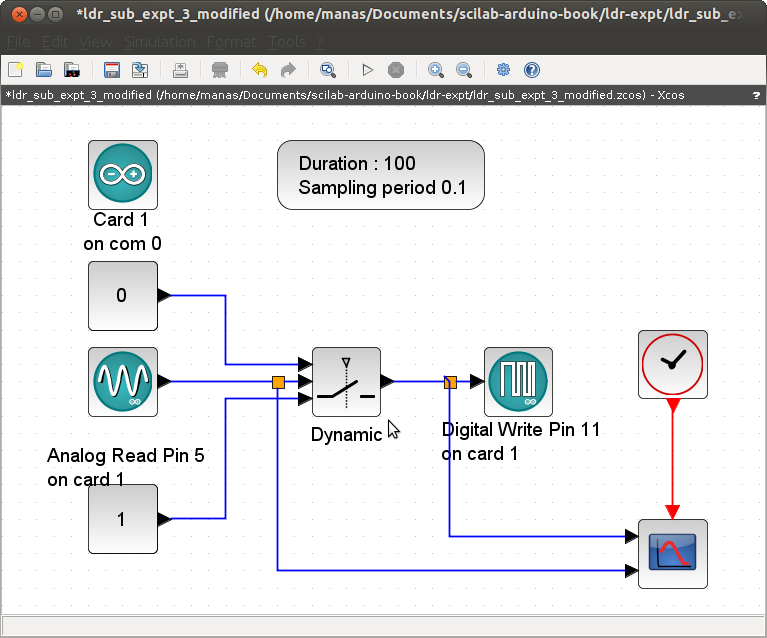
\includegraphics[width=\lgfig]{\LocLDRfig/ldr-led.png}
% \caption{Xcos diagram to change LED state depending on the LDR values}
% \label{fig:ldrxcosled}
% \end{figure}

% \begin{figure}
% \centering
% 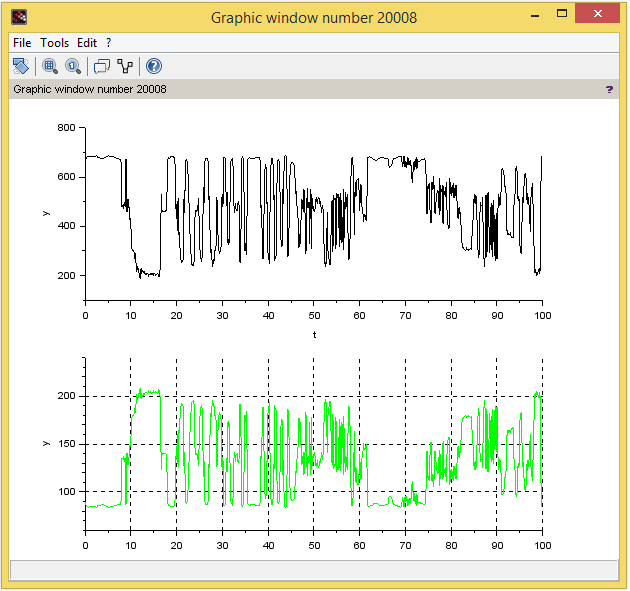
\includegraphics[width=\lgfig]{\LocLDRfig/ldr-led-out.png}
% \caption{LDR output and corresponding LED input}
% \label{fig:ldrledout}
% \end{figure}



%%%%%%%%%%%%%%python code

%%%%%%%%%%%%%%python code

%%%%%begin julia code

%%%%%end julia


%%%%%begin OpenModelica code
%%%%%%%%%%%%%%%%%OpenModelica ends
